% RLC-Serienschwingkreis - Impedanzkurve |Z|/Xk von w/w0 mit Q=1,2,3,4,1000
\def\R{10}%     10 Ohm
\def\L{10e-3}%  10 mH
\def\C{10e-6}%  10 uF
\def\Zk{31.623}% Zk = sqrt(L/C) = 31.623 Ohm
% w0 = 1/sqrt(LC) = 3162.278 Hz
% Güte Q = Zk/R -> R = Zk/Q
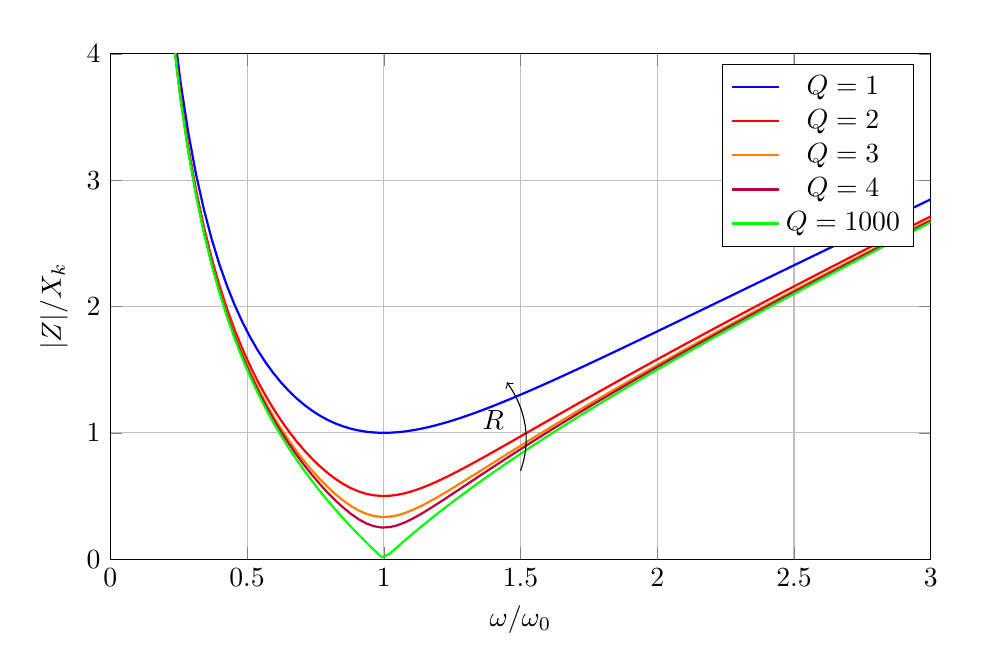
\begin{tikzpicture}[x=1cm,y=1cm]
    \draw[draw=none] (-1.05,-1) rectangle (10.75,6.75); % boundbox (not matching width and height, don't know why) % set draw=black (debug) or draw=none (final)
    \begin{axis}[
        xlabel={$\omega/\omega_0$},
        ylabel={$|Z|/X_k$},
        xmin=0, xmax=3,
        ymin=0, ymax=4,
        width=12cm,
        height=8cm,
        samples=100,
        grid=both,
        xtick={0, 0.5, 1, 1.5, 2, 2.5, 3},
    ]
    % Z/Xk = R + jXk*(w/w0 - w0/w)
    % |Z|/Xk = sqrt( (1/Q)^2 + (w/w0 - w0/w)^2 )
    \addplot[domain=0.2:3, mark=$Q=1$, thick, color=blue]     {(sqrt((1/1)^2+(x-1/x)^2))}; % Güte 1 R=31.62
    \addplot[domain=0.2:3, mark=$Q=2$, thick, color=red]      {(sqrt((1/2)^2+(x-1/x)^2))}; % Güte 2 R=15.81
    \addplot[domain=0.2:3, mark=$Q=3$, thick, color=orange]   {(sqrt((1/3)^2+(x-1/x)^2))}; % Güte 3 R=10.54
    \addplot[domain=0.2:3, mark=$Q=4$, thick, color=purple]   {(sqrt((1/4)^2+(x-1/x)^2))}; % Güte 4 R=7.91
    \addplot[domain=0.2:3, mark=$Q=1000$, thick, color=green] {(sqrt((1/1000)^2+(x-1/x)^2))}; % Güte 1000 R=0.032
    \addlegendentry{$Q=1$}
    \addlegendentry{$Q=2$}
    \addlegendentry{$Q=3$}
    \addlegendentry{$Q=4$}
    \addlegendentry{$Q=1000$}
    % R Steigend 
    \draw [->](axis cs:1.5,0.7) .. controls (axis cs:1.55,1) and (axis cs:1.5, 1.25) .. (axis cs:1.45,1.4);
    \draw(axis cs:1.4, 1.1)node{$R$};
    \end{axis}
\end{tikzpicture}